% Editorial presentation; repeated_extension.tex preserves the frozen binding.
\subsection{Repeated answers and source variation}
\label{sec:repeated-extension}

Among complete request pairs, Astra's claim-label rate differed by 0.75 for Gemini 3.1 Pro Preview and 0.22 for Claude Opus 5.5 when a self-referential instruction with a history continuation was compared with the reverse pairing. Unlike the historical panel, all four request types were randomized and interleaved in this collection. Each model supplied 32 fresh continuation pairs, with the two wording families weighted equally. Each unchanged request was submitted three times without a generation seed; neutral-instruction and donor-continuation controls were not repeated. The models were selected after the earlier panel's results.

Astra counted explicit or implicit claims of current subjective experience; Opus 5.5 provided a second automated reading. The table shows individual 97.5\% primary intervals for Astra and descriptive 95\% intervals for Opus. The conservative planned-sample bound for the Opus model includes zero. Astra labels are missing for 1 Gemini answer. Opus 5.5 labels are missing for 1 Opus answer. Missing labels remain unknown: complete-request estimates and all-planned-answer bounds are shown separately.

Even with the instruction, continuation and final question unchanged, the
three answers did not always receive the same label. For SH requests
(a self-referential instruction paired with a history continuation), we
separated two questions:
\begin{itemize}
\item \textbf{How much did labels vary across repeated answers to the same
request?} This variation, $W$, ranged from 0.16 to 0.20 across the two
response models and two automated readers.
\item \textbf{Did choosing a different history continuation add further
variation?} After accounting for the variation among repeated answers,
the additional component, $B$, was uncertain: all four descriptive
95\% intervals included zero.
\end{itemize}
Thus, one answer does not capture all the variation we observed for a fixed
request. How much more variation comes from the choice of continuation
remains unresolved. These are differences in automated labels, reflecting
both the answers and how they are scored, not a pure measure of model
randomness. Appendix~\ref{app:repeated-variation} gives the calculation
and its limitations.

\begin{table}[t]
\centering
\footnotesize
\setlength{\tabcolsep}{2pt}
\begin{tabular}{llrrll}
\toprule
\addlinespace[2pt]
Model & Reader & Available labels & \shortstack{Complete SH-HS\\blocks} & SH-HS [interval] & Missing bounds \\
\midrule
Gemini 3.1 & Astra & 383/384 & 31/32 & 0.75 [0.66, 0.84] & [0.73, 0.74] \\
Gemini 3.1 & Opus 5.5 & 384/384 & 32/32 & 0.70 [0.61, 0.77] & [0.70, 0.70] \\
Opus 5.5 & Astra & 384/384 & 32/32 & 0.22 [0.14, 0.31] & [0.22, 0.22] \\
Opus 5.5 & Opus 5.5 & 383/384 & 31/32 & 0.35 [0.24, 0.46] & [0.32, 0.33] \\
\bottomrule
\end{tabular}
\caption{SH-HS differences in label rates. Astra's primary intervals are individually 97.5\%, giving nominal 95\% coverage across the fixed two-model family; Opus intervals are descriptive 95\%. Intervals resample paired source blocks within wording family, retaining all three answers; coverage is approximate. The final column bounds missing labels over all planned blocks, not sampling uncertainty. Complete-block estimates exclude blocks with missing labels; missing-label bounds retain all 32 blocks and need not contain the complete-block estimate. S and H mean self-referential and history-focused; the first letter denotes the instruction and the second the continuation.}
\label{tab:repeated-extension}
\end{table}

\begin{figure}[t]
\centering
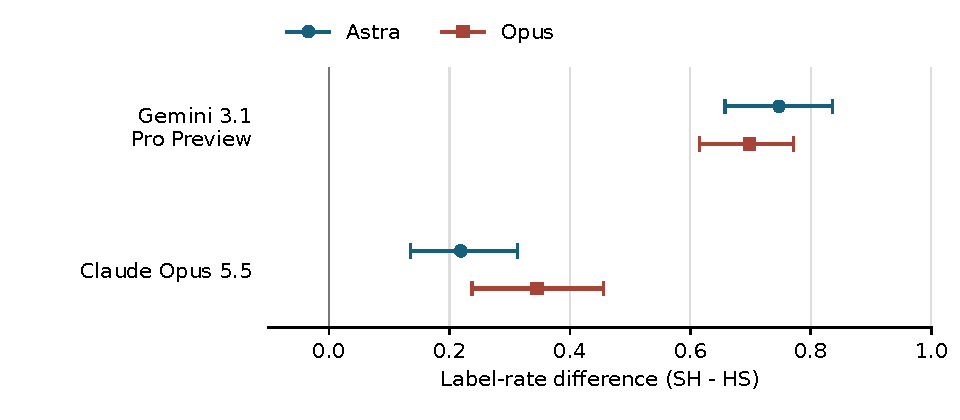
\includegraphics[width=\linewidth]{../evidence/repeated_presentation/summary.pdf}
\caption{\textbf{Instruction-advantage estimates from repeated answers.}
Each point summarizes SH--HS, counting explicit or implicit current claims;
positive values favor the retained self-referential instruction over its
continuation. Rows identify the response model; colors identify the reader
(GPT-6 Astra or Claude Opus 5.5). Bars are paired-block bootstrap intervals:
97.5\% for Astra, giving nominal 95\% coverage across the two-model primary
family, and descriptive 95\% for Opus. Coverage is approximate and conditional
on complete requests (Table~\ref{tab:repeated-extension}).
Figure~\ref{fig:repeated-variation-detail} retains the block-level detail,
variance analysis and wider conservative bounds, which include zero for
Claude Opus 5.5 responses.}
\label{fig:repeated-extension}
\end{figure}
